\begin{tikzpicture}
\pgfdeclareplotmark{cross} {
\pgfpathmoveto{\pgfpoint{-0.3\pgfplotmarksize}{\pgfplotmarksize}}
\pgfpathlineto{\pgfpoint{+0.3\pgfplotmarksize}{\pgfplotmarksize}}
\pgfpathlineto{\pgfpoint{+0.3\pgfplotmarksize}{0.3\pgfplotmarksize}}
\pgfpathlineto{\pgfpoint{+1\pgfplotmarksize}{0.3\pgfplotmarksize}}
\pgfpathlineto{\pgfpoint{+1\pgfplotmarksize}{-0.3\pgfplotmarksize}}
\pgfpathlineto{\pgfpoint{+0.3\pgfplotmarksize}{-0.3\pgfplotmarksize}}
\pgfpathlineto{\pgfpoint{+0.3\pgfplotmarksize}{-1.\pgfplotmarksize}}
\pgfpathlineto{\pgfpoint{-0.3\pgfplotmarksize}{-1.\pgfplotmarksize}}
\pgfpathlineto{\pgfpoint{-0.3\pgfplotmarksize}{-0.3\pgfplotmarksize}}
\pgfpathlineto{\pgfpoint{-1.\pgfplotmarksize}{-0.3\pgfplotmarksize}}
\pgfpathlineto{\pgfpoint{-1.\pgfplotmarksize}{0.3\pgfplotmarksize}}
\pgfpathlineto{\pgfpoint{-0.3\pgfplotmarksize}{0.3\pgfplotmarksize}}
\pgfpathclose
\pgfusepathqstroke
}
\pgfdeclareplotmark{cross*} {
\pgfpathmoveto{\pgfpoint{-0.3\pgfplotmarksize}{\pgfplotmarksize}}
\pgfpathlineto{\pgfpoint{+0.3\pgfplotmarksize}{\pgfplotmarksize}}
\pgfpathlineto{\pgfpoint{+0.3\pgfplotmarksize}{0.3\pgfplotmarksize}}
\pgfpathlineto{\pgfpoint{+1\pgfplotmarksize}{0.3\pgfplotmarksize}}
\pgfpathlineto{\pgfpoint{+1\pgfplotmarksize}{-0.3\pgfplotmarksize}}
\pgfpathlineto{\pgfpoint{+0.3\pgfplotmarksize}{-0.3\pgfplotmarksize}}
\pgfpathlineto{\pgfpoint{+0.3\pgfplotmarksize}{-1.\pgfplotmarksize}}
\pgfpathlineto{\pgfpoint{-0.3\pgfplotmarksize}{-1.\pgfplotmarksize}}
\pgfpathlineto{\pgfpoint{-0.3\pgfplotmarksize}{-0.3\pgfplotmarksize}}
\pgfpathlineto{\pgfpoint{-1.\pgfplotmarksize}{-0.3\pgfplotmarksize}}
\pgfpathlineto{\pgfpoint{-1.\pgfplotmarksize}{0.3\pgfplotmarksize}}
\pgfpathlineto{\pgfpoint{-0.3\pgfplotmarksize}{0.3\pgfplotmarksize}}
\pgfpathclose
\pgfusepathqfillstroke
}
\pgfdeclareplotmark{newstar} {
\pgfpathmoveto{\pgfqpoint{0pt}{\pgfplotmarksize}}
\pgfpathlineto{\pgfqpointpolar{44}{0.5\pgfplotmarksize}}
\pgfpathlineto{\pgfqpointpolar{18}{\pgfplotmarksize}}
\pgfpathlineto{\pgfqpointpolar{-20}{0.5\pgfplotmarksize}}
\pgfpathlineto{\pgfqpointpolar{-54}{\pgfplotmarksize}}
\pgfpathlineto{\pgfqpointpolar{-90}{0.5\pgfplotmarksize}}
\pgfpathlineto{\pgfqpointpolar{234}{\pgfplotmarksize}}
\pgfpathlineto{\pgfqpointpolar{198}{0.5\pgfplotmarksize}}
\pgfpathlineto{\pgfqpointpolar{162}{\pgfplotmarksize}}
\pgfpathlineto{\pgfqpointpolar{134}{0.5\pgfplotmarksize}}
\pgfpathclose
\pgfusepathqstroke
}
\pgfdeclareplotmark{newstar*} {
\pgfpathmoveto{\pgfqpoint{0pt}{\pgfplotmarksize}}
\pgfpathlineto{\pgfqpointpolar{44}{0.5\pgfplotmarksize}}
\pgfpathlineto{\pgfqpointpolar{18}{\pgfplotmarksize}}
\pgfpathlineto{\pgfqpointpolar{-20}{0.5\pgfplotmarksize}}
\pgfpathlineto{\pgfqpointpolar{-54}{\pgfplotmarksize}}
\pgfpathlineto{\pgfqpointpolar{-90}{0.5\pgfplotmarksize}}
\pgfpathlineto{\pgfqpointpolar{234}{\pgfplotmarksize}}
\pgfpathlineto{\pgfqpointpolar{198}{0.5\pgfplotmarksize}}
\pgfpathlineto{\pgfqpointpolar{162}{\pgfplotmarksize}}
\pgfpathlineto{\pgfqpointpolar{134}{0.5\pgfplotmarksize}}
\pgfpathclose
\pgfusepathqfillstroke
}
\definecolor{c}{rgb}{1,1,1};
\draw [color=c, fill=c] (0,0) rectangle (20,14.4361);
\draw [color=c, fill=c] (3.2,2.30977) rectangle (19,13.7143);
\definecolor{c}{rgb}{0,0,0};
\draw [c,line width=0.9] (3.2,2.30977) -- (3.2,13.7143) -- (19,13.7143) -- (19,2.30977) -- (3.2,2.30977);
\definecolor{c}{rgb}{0.1802,0.7178,0.6425};
\draw [color=c, fill=c] (3.2,2.30977) rectangle (6.53333,4.44812);
\definecolor{c}{rgb}{0.453559,0.742331,0.504766};
\draw [color=c, fill=c] (6.53333,2.30977) rectangle (9.86667,4.44812);
\definecolor{c}{rgb}{0.956881,0.774519,0.230291};
\draw [color=c, fill=c] (9.86667,2.30977) rectangle (12.3333,4.44812);
\draw [color=c, fill=c] (13.3333,2.30977) rectangle (16.5333,4.44812);
\definecolor{c}{rgb}{0.9842,0.903169,0.111953};
\draw [color=c, fill=c] (16.5333,2.30977) rectangle (19,4.44812);
\definecolor{c}{rgb}{0.1802,0.7178,0.6425};
\draw [color=c, fill=c] (3.2,4.44812) rectangle (6.53333,5.87368);
\definecolor{c}{rgb}{0.116419,0.686966,0.702991};
\draw [color=c, fill=c] (6.53333,4.44812) rectangle (9.86667,5.87368);
\definecolor{c}{rgb}{0.322347,0.730556,0.570878};
\draw [color=c, fill=c] (9.86667,4.44812) rectangle (12.3333,5.87368);
\definecolor{c}{rgb}{0.956881,0.774519,0.230291};
\draw [color=c, fill=c] (13.3333,4.44812) rectangle (16.5333,5.87368);
\definecolor{c}{rgb}{0.977,0.977044,0.0583656};
\draw [color=c, fill=c] (16.5333,4.44812) rectangle (19,5.87368);
\definecolor{c}{rgb}{0.0526375,0.656131,0.763481};
\draw [color=c, fill=c] (3.2,5.87368) rectangle (6.53333,8.01203);
\draw [color=c, fill=c] (6.53333,5.87368) rectangle (9.86667,8.01203);
\definecolor{c}{rgb}{0.116419,0.686966,0.702991};
\draw [color=c, fill=c] (9.86667,5.87368) rectangle (12.3333,8.01203);
\definecolor{c}{rgb}{0.701397,0.739462,0.397147};
\draw [color=c, fill=c] (13.3333,5.87368) rectangle (16.5333,8.01203);
\definecolor{c}{rgb}{0.956881,0.774519,0.230291};
\draw [color=c, fill=c] (16.5333,5.87368) rectangle (19,8.01203);
\definecolor{c}{rgb}{0.0526375,0.656131,0.763481};
\draw [color=c, fill=c] (3.2,8.01203) rectangle (6.53333,13.7143);
\definecolor{c}{rgb}{0.033475,0.616063,0.800231};
\draw [color=c, fill=c] (6.53333,8.01203) rectangle (9.86667,13.7143);
\definecolor{c}{rgb}{0.0526375,0.656131,0.763481};
\draw [color=c, fill=c] (9.86667,8.01203) rectangle (12.3333,13.7143);
\definecolor{c}{rgb}{0.701397,0.739462,0.397147};
\draw [color=c, fill=c] (13.3333,8.01203) rectangle (16.5333,13.7143);
\definecolor{c}{rgb}{0.8186,0.7328,0.3499};
\draw [color=c, fill=c] (16.5333,8.01203) rectangle (19,13.7143);
\definecolor{c}{rgb}{0,0,0};
\draw (4.86667,3.37895) node[scale=1.61424, color=c, rotate=1]{$\genfrac{}{}{0pt}{}{1.271}{\pm 0.019}$};
\draw (8.2,3.37895) node[scale=1.61424, color=c, rotate=1]{$\genfrac{}{}{0pt}{}{1.509}{\pm 0.003}$};
\draw (11.1,3.37895) node[scale=1.61424, color=c, rotate=1]{$\genfrac{}{}{0pt}{}{2.142}{\pm 0.004}$};
\draw (14.9333,3.37895) node[scale=1.61424, color=c, rotate=1]{$\genfrac{}{}{0pt}{}{2.154}{\pm 0.023}$};
\draw (17.7667,3.37895) node[scale=1.61424, color=c, rotate=1]{$\genfrac{}{}{0pt}{}{2.465}{\pm 0.023}$};
\draw (4.86667,5.1609) node[scale=1.61424, color=c, rotate=1]{$\genfrac{}{}{0pt}{}{1.196}{\pm 0.012}$};
\draw (8.2,5.1609) node[scale=1.61424, color=c, rotate=1]{$\genfrac{}{}{0pt}{}{1.176}{\pm 0.021}$};
\draw (11.1,5.1609) node[scale=1.61424, color=c, rotate=1]{$\genfrac{}{}{0pt}{}{1.424}{\pm 0.059}$};
\draw (14.9333,5.1609) node[scale=1.61424, color=c, rotate=1]{$\genfrac{}{}{0pt}{}{2.125}{\pm 0.022}$};
\draw (17.7667,5.1609) node[scale=1.61424, color=c, rotate=1]{$\genfrac{}{}{0pt}{}{2.648}{\pm 0.024}$};
\draw (4.86667,6.94286) node[scale=1.61424, color=c, rotate=1]{$\genfrac{}{}{0pt}{}{0.937}{\pm 0.008}$};
\draw (8.2,6.94286) node[scale=1.61424, color=c, rotate=1]{$\genfrac{}{}{0pt}{}{1.000}{\pm 0.008}$};
\draw (11.1,6.94286) node[scale=1.61424, color=c, rotate=1]{$\genfrac{}{}{0pt}{}{1.113}{\pm 0.013}$};
\draw (14.9333,6.94286) node[scale=1.61424, color=c, rotate=1]{$\genfrac{}{}{0pt}{}{1.832}{\pm 0.017}$};
\draw (17.7667,6.94286) node[scale=1.61424, color=c, rotate=1]{$\genfrac{}{}{0pt}{}{2.138}{\pm 0.019}$};
\draw (4.86667,10.8632) node[scale=1.61424, color=c, rotate=1]{$\genfrac{}{}{0pt}{}{0.930}{\pm 0.023}$};
\draw (8.2,10.8632) node[scale=1.61424, color=c, rotate=1]{$\genfrac{}{}{0pt}{}{0.908}{\pm 0.045}$};
\draw (11.1,10.8632) node[scale=1.61424, color=c, rotate=1]{$\genfrac{}{}{0pt}{}{0.941}{\pm 0.032}$};
\draw (14.9333,10.8632) node[scale=1.61424, color=c, rotate=1]{$\genfrac{}{}{0pt}{}{1.780}{\pm 0.042}$};
\draw (17.7667,10.8632) node[scale=1.61424, color=c, rotate=1]{$\genfrac{}{}{0pt}{}{1.952}{\pm 0.061}$};
\draw [c,line width=0.9] (3.2,2.30977) -- (19,2.30977);
\draw [anchor=north] (4.86667,2.13871) node[scale=1.0576, color=c, rotate=0]{[0.0 - 0.5]};
\draw [anchor=north] (8.2,2.13871) node[scale=1.0576, color=c, rotate=0]{[0.5 - 1.0]};
\draw [anchor=north] (11.1,2.13871) node[scale=1.0576, color=c, rotate=0]{[1.0 - 1.37]};
% \draw [anchor=north] (12.8333,2.13871) node[scale=1.0576, color=c, rotate=0]{[1.37 - 1.52]};
\draw [anchor=north] (14.9333,2.13871) node[scale=1.0576, color=c, rotate=0]{[1.52 - 2.0]};
\draw [anchor=north] (17.7667,2.13871) node[scale=1.0576, color=c, rotate=0]{[2.0 - 2.37]};
\draw [c,line width=0.9] (3.2,2.65191) -- (3.2,2.30977);
\draw [c,line width=0.9] (6.53333,2.65191) -- (6.53333,2.30977);
\draw [c,line width=0.9] (9.86667,2.65191) -- (9.86667,2.30977);
\draw [c,line width=0.9] (13.2,2.65191) -- (13.2,2.30977);
\draw [c,line width=0.9] (16.5333,2.65191) -- (16.5333,2.30977);
\draw [c,line width=0.9] (16.5333,2.65191) -- (16.5333,2.30977);
\draw [anchor= east] (19,0.692932) node[scale=1.61424, color=c, rotate=0]{$|\eta|_{  e}^{probe}$};
\draw [c,line width=0.9] (3.2,13.7143) -- (19,13.7143);
\draw [c,line width=0.9] (3.2,13.3722) -- (3.2,13.7143);
\draw [c,line width=0.9] (6.53333,13.3722) -- (6.53333,13.7143);
\draw [c,line width=0.9] (9.86667,13.3722) -- (9.86667,13.7143);
\draw [c,line width=0.9] (13.2,13.3722) -- (13.2,13.7143);
\draw [c,line width=0.9] (16.5333,13.3722) -- (16.5333,13.7143);
\draw [c,line width=0.9] (16.5333,13.3722) -- (16.5333,13.7143);
\draw [c,line width=0.9] (3.2,2.30977) -- (3.2,13.7143);
\draw [anchor= east] (2.963,3.37895) node[scale=1.0576, color=c, rotate=0]{[20 - 35] };
\draw [anchor= east] (2.963,5.1609) node[scale=1.0576, color=c, rotate=0]{[35 - 45] };
\draw [anchor= east] (2.963,6.94286) node[scale=1.0576, color=c, rotate=0]{[45 - 60] };
\draw [anchor= east] (2.963,8.6) node[scale=1.0576, color=c, rotate=0]{[60 - 100]};
\draw [c,line width=0.9] (3.674,2.30977) -- (3.2,2.30977);
\draw [c,line width=0.9] (3.674,5.1609) -- (3.2,5.1609);
\draw [c,line width=0.9] (3.674,8.01203) -- (3.2,8.01203);
\draw [c,line width=0.9] (3.674,10.8632) -- (3.2,10.8632);
\draw [c,line width=0.9] (3.674,13.7143) -- (3.2,13.7143);
\draw [anchor= east] (0.96,13.7143) node[scale=1.61424, color=c, rotate=90]{$p_{T,  e}^{probe}  [GeV]$};
\draw [c,line width=0.9] (19,2.30977) -- (19,13.7143);
\draw [c,line width=0.9] (18.526,2.30977) -- (19,2.30977);
\draw [c,line width=0.9] (18.526,5.1609) -- (19,5.1609);
\draw [c,line width=0.9] (18.526,8.01203) -- (19,8.01203);
\draw [c,line width=0.9] (18.526,10.8632) -- (19,10.8632);
\draw [c,line width=0.9] (18.526,13.7143) -- (19,13.7143);
\definecolor{c}{rgb}{0.150523,0.241303,0.660565};
\draw [color=c, fill=c] (19.1,2.30977) rectangle (19.99,2.88);
\definecolor{c}{rgb}{0.0880387,0.322448,0.802768};
\draw [color=c, fill=c] (19.1,2.88) rectangle (19.99,3.45023);
\definecolor{c}{rgb}{0.0633125,0.391444,0.861859};
\draw [color=c, fill=c] (19.1,3.45023) rectangle (19.99,4.02045);
\definecolor{c}{rgb}{0.0703625,0.445519,0.850647};
\draw [color=c, fill=c] (19.1,4.02045) rectangle (19.99,4.59068);
\definecolor{c}{rgb}{0.078,0.5041,0.8385};
\draw [color=c, fill=c] (19.1,4.59068) rectangle (19.99,5.1609);
\definecolor{c}{rgb}{0.0557375,0.560081,0.819366};
\draw [color=c, fill=c] (19.1,5.1609) rectangle (19.99,5.73113);
\definecolor{c}{rgb}{0.033475,0.616063,0.800231};
\draw [color=c, fill=c] (19.1,5.73113) rectangle (19.99,6.30135);
\definecolor{c}{rgb}{0.0526375,0.656131,0.763481};
\draw [color=c, fill=c] (19.1,6.30135) rectangle (19.99,6.87158);
\definecolor{c}{rgb}{0.116419,0.686966,0.702991};
\draw [color=c, fill=c] (19.1,6.87158) rectangle (19.99,7.4418);
\definecolor{c}{rgb}{0.1802,0.7178,0.6425};
\draw [color=c, fill=c] (19.1,7.4418) rectangle (19.99,8.01203);
\definecolor{c}{rgb}{0.322347,0.730556,0.570878};
\draw [color=c, fill=c] (19.1,8.01203) rectangle (19.99,8.58226);
\definecolor{c}{rgb}{0.453559,0.742331,0.504766};
\draw [color=c, fill=c] (19.1,8.58226) rectangle (19.99,9.15248);
\definecolor{c}{rgb}{0.584194,0.746125,0.444394};
\draw [color=c, fill=c] (19.1,9.15248) rectangle (19.99,9.72271);
\definecolor{c}{rgb}{0.701397,0.739462,0.397147};
\draw [color=c, fill=c] (19.1,9.72271) rectangle (19.99,10.2929);
\definecolor{c}{rgb}{0.8186,0.7328,0.3499};
\draw [color=c, fill=c] (19.1,10.2929) rectangle (19.99,10.8632);
\definecolor{c}{rgb}{0.884975,0.752825,0.292488};
\draw [color=c, fill=c] (19.1,10.8632) rectangle (19.99,11.4334);
\definecolor{c}{rgb}{0.956881,0.774519,0.230291};
\draw [color=c, fill=c] (19.1,11.4334) rectangle (19.99,12.0036);
\definecolor{c}{rgb}{0.992,0.823138,0.170006};
\draw [color=c, fill=c] (19.1,12.0036) rectangle (19.99,12.5738);
\definecolor{c}{rgb}{0.9842,0.903169,0.111953};
\draw [color=c, fill=c] (19.1,12.5738) rectangle (19.99,13.1441);
\definecolor{c}{rgb}{0.977,0.977044,0.0583656};
\draw [color=c, fill=c] (19.1,13.1441) rectangle (19.99,13.7143);
\definecolor{c}{rgb}{0,0,0};
\draw [c,line width=0.9] (19.99,2.30977) -- (19.99,13.7143);
\draw [c,line width=0.9] (19.516,2.30977) -- (19.99,2.30977);
\draw [c,line width=0.9] (19.516,4.4636) -- (19.99,4.4636);
\draw [c,line width=0.9] (19.516,6.61742) -- (19.99,6.61742);
\draw [c,line width=0.9] (19.516,8.77124) -- (19.99,8.77124);
\draw [c,line width=0.9] (19.516,10.9251) -- (19.99,10.9251);
\draw [c,line width=0.9] (19.516,13.0789) -- (19.99,13.0789);
\draw [c,line width=0.9] (19.516,13.0789) -- (19.99,13.0789);
\draw [anchor= west] (20.09,2.30977) node[scale=1.61424, color=c, rotate=0]{0};
\draw [anchor= west] (20.09,4.4636) node[scale=1.61424, color=c, rotate=0]{0.5};
\draw [anchor= west] (20.09,6.61742) node[scale=1.61424, color=c, rotate=0]{1};
\draw [anchor= west] (20.09,8.77124) node[scale=1.61424, color=c, rotate=0]{1.5};
\draw [anchor= west] (20.09,10.9251) node[scale=1.61424, color=c, rotate=0]{2};
\draw [anchor= west] (20.09,13.0789) node[scale=1.61424, color=c, rotate=0]{2.5};
\end{tikzpicture}
